\tikzposterlatexaffectionproofoff
\usetheme{Default}

\definecolor{text}{HTML}{e0e4f7}
\definecolor{background}{HTML}{111116}
\definecolor{boxes}{HTML}{2a2a32}
\definecolor{unired}{HTML}{a51e37}

\colorlet{blocktitlefgcolor}{text}
\colorlet{backgroundcolor}{background}
\colorlet{blocktitlebgcolor}{background}
\colorlet{blockbodyfgcolor}{text}
\colorlet{innerblocktitlebgcolor}{background}
\colorlet{innerblocktitlefgcolor}{text}
\colorlet{notefrcolor}{text}
\colorlet{notefgcolor}{background}
\colorlet{notebgcolor}{background}


% Title setup
\settitle{
% Rearrange the order of the minipages to e.g. center the title between the logos
\begin{minipage}[c]{0.8\paperwidth}
%    \centering
    \vspace{2.5cm}\hspace{1.5cm}
    \color{text}{\Huge{\textbf{\@title}} \par}
    \vspace*{2em}\hspace{1.5cm}
    \color{text}{\LARGE \@author \par}
    \vspace*{2em}\hspace{1.5cm}
    \color{text}{\Large \@institute}
    \vspace{2.5cm}
\end{minipage}
\begin{minipage}[c]{0.2\paperwidth}
    \centering
    % \vspace{1cm}
    \hspace{-7cm}
    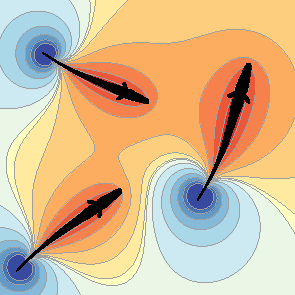
\includegraphics[width=0.7\linewidth]{figs/efishlogo.pdf}
\end{minipage}}
% \begin{minipage}[c]{0.2\paperwidth}
%     \vspace{1cm}\hspace{1cm}
%     \centering
%     \includegraphics[width=\linewidth]{example-image-a}
% \end{minipage}}

% define title style with background box (currently white)
\definetitlestyle{sampletitle}{
    width=841mm,
    roundedcorners=0,
    linewidth=0pt,
    innersep=15pt,
    titletotopverticalspace=0mm,
    titletoblockverticalspace=5pt
}{
    \begin{scope}[line width=\titlelinewidth,
        rounded corners=\titleroundedcorners]
    \draw[fill=text, color=boxes]
    (\titleposleft,\titleposbottom)
    rectangle
    (\titleposright,\titlepostop);
    \end{scope}
}

% define coustom block style for visible blocks
\defineblockstyle{GrayBlock}{
    titlewidthscale=1,
    bodywidthscale=1,
    % titlecenter,
    titleleft,
    titleoffsetx=0pt,
    titleoffsety=-30pt,
    bodyoffsetx=0pt,
    bodyoffsety=-40pt,
    bodyverticalshift=0mm,
    roundedcorners=25,
    linewidth=1pt,
    titleinnersep=20pt,
    bodyinnersep=38pt
}{
    \draw[rounded corners=\blockroundedcorners, inner sep=\blockbodyinnersep,
          line width=\blocklinewidth, color=background,
          top color=boxes, bottom color=boxes,
          ]
      (blockbody.south west) rectangle (blockbody.north east); %
    \ifBlockHasTitle%
        \draw[rounded corners=\blockroundedcorners, inner sep=\blocktitleinnersep,
          top color=background, bottom color=background,
          line width=2, color=background, %fill=blocktitlebgcolor
          ]
      (blocktitle.south west) rectangle (blocktitle.north east); %
    \fi%
}
\newcommand\myblock[3][GrayBlock]{\useblockstyle{#1}\block{#2}{#3}\useblockstyle{Default}}

% Define blockstyle for tranparent block
\defineblockstyle{TranspBlock}{
    titlewidthscale=0.99,
    bodywidthscale=0.99,
    titleleft,
    titleoffsetx=15pt,
    titleoffsety=-40pt,
    bodyoffsetx=0pt,
    bodyoffsety=-40pt,
    bodyverticalshift=0mm,
    roundedcorners=25,
    linewidth=1pt,
    titleinnersep=20pt,
    bodyinnersep=38pt
}{
    \draw[rounded corners=\blockroundedcorners, inner sep=\blockbodyinnersep,
          line width=\blocklinewidth, color=background,
          top color=background, bottom color=background,
          ]
      (blockbody.south west) rectangle (blockbody.north east); %
    \ifBlockHasTitle%
        \draw[rounded corners=\blockroundedcorners, inner sep=\blocktitleinnersep,
          top color=background, bottom color=background,
          line width=2, color=background, %fill=blocktitlebgcolor
          ]
      (blocktitle.south west) rectangle (blocktitle.north east); %
    \fi%
}
\renewcommand\myblock[3][TranspBlock]{\useblockstyle{#1}\block{#2}{#3}\useblockstyle{Default}}
